% !TEX root = ../main.tex

\chapter{编译链实现与评估} \label{ch:implement}

\section{编译链概览} \label{sec:overview}

我们构建了一个从函数式语言PCF到LLVM IR的部分经过验证的编译器,并在Coq定理证明工具中
完成了编译算法和形式化验证的实现~\cite{chlipala2022certified}。
在本章中,我们主要是从高层次的角度介绍了这个编译器原型,省略了转换算法设计和证明定理的详细信息。
CPS转换及CPS到SSA转换的正确性通过源程序和目标程序之间的模拟进行形式化验证,
遵循第\ref{sec:compcertbackend}节中所介绍的CompCert后端的验证框架。
我们使用$\approx $表示语义保存性质。PCF、CPS和SSA的程序分别表示为$t_{pcf}$、$t_{cps}$和$t_{ssa}$。
通过对$t_{pcf}\approx t_{cps}$和$t_{cps}\approx t_{ssa}$的形式化证明,可以组合推导出$t_{pcf}\approx t_{ssa}$。
然后我们就得到了一个从PCF到SSA的经验证的编译过程。我们应用该经验证的编译过程,构建出一个编译器原型。
该编译器读取PCF程序,并经过图\ref{overview}中所示的几个编译步骤生成LLVM IR程序。

\begin{figure}[htbp]
    \centering
    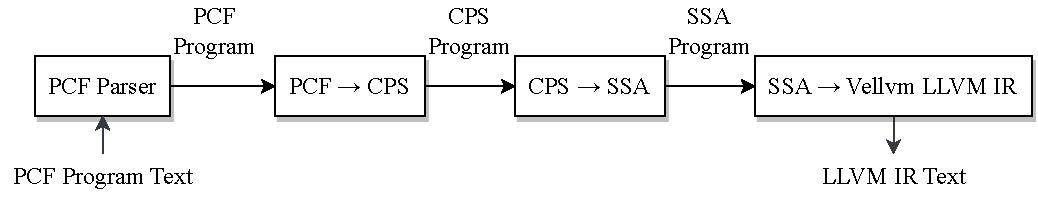
\includegraphics[width=0.8\linewidth]{figures/overview.pdf}
    \caption{PCF到LLVM编译链概览}\label{overview}
\end{figure}

\subsection{PCF语法分析器}

该PCF语法分析器(Parser)将文本形式的PCF程序提取为Coq中的结构化PCF代码项。
为了分析文本信息并提取PCF程序,获取源程序的语法结构至关重要。对于文本形式的PCF程序,
我们首先用词法分析器(Lexical Parser)将其解析为令牌(Token)流。
随后,使用语法分析器(Syntax Parser)分析该令牌流,生成Coq中的直接风格PCF程序项的抽象语法树。

\subsection{CPS转换}

如第\ref{sec:background}节中所言,函数式编程语言的编译器通常会将直接风格的程序转换为CPS形式,以获得显式的控制流。
我们已经得到了PCF程序的抽象语法树,但它是直接风格的程序,所以接下来需要使用CPS转换将其编译为CPS风格的程序。
将直接风格的PCF程序转换为CPS形式的算法主要由当前代码项和当前项被规约为某个值后要处理的下一个项决定。
另外,我们为直接风格及CPS风格的PCF语言定义了小步操作语义,并证明了CPS转换的前向模拟性质。
关于该CPS转换算法及其正确性验证的详细信息将在第\ref{sec:cpstrans}节和第\ref{sec:cpsforward}节中进行讨论。

\subsection{从CPS到SSA}

该编译链中最关键的部分是从CPS风格的函数式程序到目标SSA程序的转换及验证。
目标SSA语言是LLVM IR的简化版本,保留了其最基本的结构和程序语句。
通过该编译过程,输入的CPS程序项将被转换为一个包含主函数的SSA程序。
同样的,我们为这种SSA语言定义了小步操作语义,并证明了从CPS到SSA转换的前向模拟。
完成这一步证明后,我们将正向模拟组合起来,并完成了从源程序到SSA程序后向模拟的证明。
在第\ref{sec:cpsssatrans}节中将详细介绍该转换算法的设计和细节。
第\ref{sec:cpsssaforward}节中将进行CPS到SSA转换算法的形式化验证,并通过运行一个示例程序展示前向模拟的每一个关键步骤。

\subsection{从SSA到LLVM IR}

上一步中得到的SSA程序被转换为Vellvm中的抽象语法树,然后转换为LLVM IR程序文本。
在该编译链中,我们使用了经过验证的LLVM基础设施Vellvm~\cite{zakowski2021modular}。
利用其在Coq实现的LLVM IR的抽象语法树,我们可以进一步输出最终的LLVM IR程序。
由于我们使用的SSA语言是LLVM IR的简化版本,它保留了LLVM IR程序的基本结构,
可以方便地编译到Vellvm中的抽象语法树。这种SSA语言省略了LLVM IR中的大部分参数。
例如,函数定义在LLVM中非常复杂,有很多可选的参数,而本文中的SSA语言只保留了函数定义中必须指定的内容。
LLVM中的表达式类型多种多样,其中整数包括多种宽度的i16、i32等,
而本文的SSA语言简化为没有明确指定类型的无限宽自然数。
该编译过程的主要工作其实就是为这些被省略的参数选取正确的默认值。


\section{编译算法及定理证明的实现}

如第~\ref{sec:overview}节中所述,我们主要使用了交互式定理证明器Coq实现
程序语言定义及编译算法,并完成相关定理的形式化证明。
Coq主要是用OCaml语言实现的,它支持数学断言的表示,并且能够检查这些断言的证明,
从其形式化的构造证明中提取出验证程序~\cite{paulin2011introduction}。
作为一种编程语言,Coq是一种依赖类型的函数式编程语言;作为一种逻辑系统,它实现了一种高阶类型理论。
也就是说,证明即是程序。

其中,编译链的PCF语法分析器(Parser)部分在OCaml中实现,它分析PCF程序文本并
在顶层Coq模块中添加需要进行编译的PCF源程序。我们在本章第~\ref{sec:pcfparser}节对其进行了介绍。
我们在Coq中完成了PCF、CPS和SSA程序语言的定义以及从PCF源程序到Vellvm抽象语法树的编译链。
这些编译过程和证明主要通过函数和模式匹配(Pattern Match)、
表示推理规则的归纳类型(Inductive)、一阶逻辑(First-Order Logic)谓词等实现。
Coq并没有提供通常的原子数据类型(布尔值、整数、字符串等),而是提供了一个机制来定义新的数据类型。
当然,Coq有强大的标准库,其中包含了许多常见数据结构的定义。
在后文中我们会详细介绍在Coq中对经验证编译链进行实现的过程。
不过,在本章中关于Coq实现代码的示例中,我们关注的是其整体结构,而不是第~\ref{ch:trans}章和第~\ref{ch:verify}章
中已经详细介绍过的定义、算法和定理等。所以,我们会省略掉大部分的具体实现内容。

\subsection{PCF语法分析器} \label{sec:pcfparser}
我们没有直接去编写实现词法解析和语法解析功能的OCaml代码,而是
使用ocamllex和ocamlyacc~\cite{smith2007ocamllex}作为词法和语法解析器的生成器。
它们的用法类似于C语言环境中的lex和yacc~\cite{levine1992lex}。
该PCF语法分析器的结构如图~\ref{fig:parser}所示。

Ocamllex可以从附加了语义行为的正则表达式(Regular Expression)集合中生成词法分析器。
我们首先在\textit{lexer.mll}中定义了直接风格PCF语言的词法解析规则,
包括输入文本中各种词法单元的模式匹配和对应的操作,然后使用ocamllex
生成词法分析器的OCaml代码\textit{lexer.ml}。
在\textit{lexer.ml}文件中,词法分析函数将词法分析缓冲区(Lexer Buffer)作为参数,
生成标记流(Tokens)。
词法分析缓冲区是在OCaml标准库模块Lexing中实现的抽象数据类型,它维护分析函数当前的状态,
并可以从输入获取内容对缓冲区进行填充~\cite{leroy2021ocaml}。
分析函数会将缓冲区中的字符与词法规则中定义的正则表达式进行匹配,直到输入的前缀符合某条规则,
执行相应的操作。如果符合多条规则,就按照最长匹配原则。
Ocamlyacc会根据语法规则\textit{grammar.mly}生成语法分析器的接口\textit{grammar.mli}
和实现\textit{grammar.ml}。语法解析函数的参数包括上文中提到的词法分析器和词法分析缓冲区。
它将词法分析得到的标记流解析为抽象语法树。之后,我们使用\textit{printer.ml}读入PCF程序
在OCaml中的抽象语法树打印出它的Coq程序并将其写入Coq编译链的顶层模块,这样就可以直接在Coq中使用它了。

\begin{figure}[htbp]
    \centering
    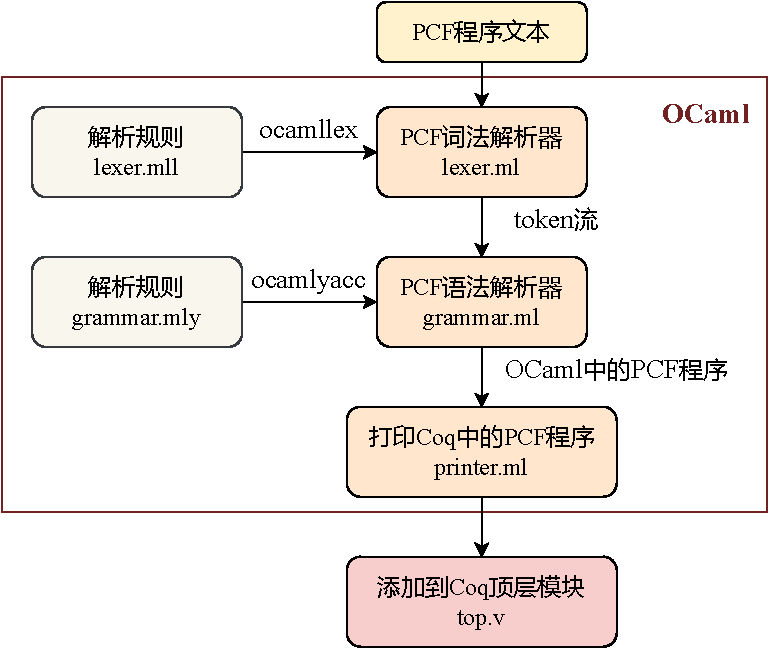
\includegraphics[width=0.7\linewidth]{figures/pcfparser.pdf}
    \caption{PCF语法分析器结构}\label{fig:parser}
\end{figure}

\subsection{程序语言定义}

如上一节所述,我们已经使用PCF语法分析器在Coq顶层编译模块得到了PCF程序的抽象语法树。
除了PCF语言的抽象语法树定义,我们还为其在Coq中实现了第~\ref{sec:cps}节中定义的小步操作语义。
我们使用Inductive类型完成了这种程序状态转换规则的定义。

\begin{lstlisting}[language=Coq]
    Inductive  pcf_term : Set  := ...
    Record  pcf_state  :=  mk_state {t : pcf_term;  ctx : context;}.
    Inductive  pcf_step : pcf_state -> pcf_state -> Prop  := ...
\end{lstlisting}

在编译算法正确性证明过程中使用的小步操作语义是关系型的,即表示为两个程序状态之间的关系。
这样的设计对于证明来说很方便,但是无法直接运行程序得到结果。
为了对操作语义和转换算法进行初步测试,使用Coq为三种语言分别构建解释器(Interpreter),
从而能够执行相应的程序,得到程序返回的结果。其中,发散的定义要取决于对最大步数的限定,即解释器的fuel。
解释器每走一步都会消耗一个fuel,如果fuel消耗完程序还没有终止或出错,就可以认为程序发散了,返回超时状态(Timeout)。
进行解释器测试主要是为了找出操作语义和转换算法中的问题,为接下来的证明减少阻碍。形式化验证过程本身与解释器没有关系。

\begin{lstlisting}[language=Coq]
    Inductive  pcf_result : Type  := 
        |  terminate : nat  ->  pcf_result 
        |  error : pcf_result
        |  timeout : pcf_result
    Fixpoint  pcf_interpreter  (fuel : nat)  (state : pcf_state) : 
        pcf_result  :=  let  'mk_state  term ctx  :=  state  in
                            match fuel with 
                                | 0  =>  timeout 
                                | S fuel'  =>  match  term, ctx  with ...
\end{lstlisting}

与PCF语言类似,我们为CPS与SSA语言也像这样完成了其语法、语义及解释器在Coq中的实现。

\subsection{转换算法的实现}

CPS转换算法~\ref{algo:cpstrans}和CPS到SSA的转换算法~\ref{cps2ssa}均在Coq中进行实现。
对于CPS转换,我们需要根据已有的变量名称列表生成新变量,且新变量不能与已有的变量名重复。
在具体实现时,我们采用的算法是为新生成的变量维护一个后缀最大值$n$。
当需要生成一个新的变量名时,我们首先尝试将前缀字符串后连接后缀$n$,并将后缀最大值加一。
这样一个字符串虽然不会与新生成的变量名冲突,但是可能会和CPS程序原有的变量名冲突。
由于我们的CPS转换算法会持续记录已有的变量名列表$l_v$,我们还需要使之与$l_v$中的
变量比较。如果产生冲突,需要重复上一步。
对于CPS到SSA的转换算法,我们首先需要实现插入指令、基本代码块、函数的$\mathbf{app}$操作。
然后,我们需要能够根据已处理的条件语句数量$n$生成新的基本代码块标签的操作fresh\_block\_label。
之后,我们就可以实现~\ref{sec:cpsssatrans}节中的转换算法了。

\begin{lstlisting}[language=Coq]  
    Definition  app_i  (i : instruction)  (t : ssa_term)  (p : pc)  : 
        ssa_term  := ... 
    Definition  fresh_block_label  (n : nat)  :  string  := ...
    Definition  G_state  :  Type  :=  (ssa_term  *  nat  *  loc_cps).
    Fixpoint  G  (t_cps : cps_term)  (t_ssa : ssa_term)  (p : pc)  
        (n : nat)  (loc : loc_cps)  :  G_state  := ...
    Definition  G_prog  (t_cps : cps_term)  :  ssa_term  := ...
\end{lstlisting}

我们还实现了从SSA到Vellvm抽象语法树的编译过程。
将Vellvm作为子模块使用,该转换步骤的目标语言是Vellvm在\textit{Syntax.LLVMAst}文件中定义的LLVM IR。
正如我们在介绍SSA语言时所说,该SSA保留了LLVM IR程序的结构。
此步转换主要是进行结构上的映射,顺便为被省略的参数选取正确的默认值。
例如,我们可以直接把SSA中的函数调用指令$x = \mathbf{call}\; f\; v$转换为LLVM AST中的
INSTR\_Op指令,但是需要为其指定$f$和$v$的类型。在这里我们统一使用64位无符号整型。
其他结构同理,基本代码块转换为LLVMAst.block,函数转换为definition,顶层翻译单元转换为toplevel\_entities。
得到Vellvm中的抽象语法树后,就可以利用其提供的工具进行LLVM程序的输出或使用LLVM后续的编译过程了。

\subsection{定理证明的实现}

完成了程序语言小步操作语义的定义和编译算法的实现,我们就可以对第~\ref{ch:verify}节中
介绍的相关定理进行证明了。
由于两步转换的前向模拟证明结构相似,此处以CPS到SSA的转换为例。

首先,我们需要定义CPS与SSA程序状态之间的不变式match\_state以及度量函数measure。
那么,定理~\ref{trm:simustep2}在Coq中就可以表示为simulation\_step。
我们使用归纳证明(Proof by Induction)的方法对simulation\_step进行证明。
如下方代码所示,我们对CPS程序状态进行一步转换所遵循的小步操作语义规则进行归纳,即Hstep。
这样,我们证明的目标就按照不同的转换规则分成了很多个子目标(Subgoal)。
在每个子目标中,我们可以根据具体的Hstep规则构造出相应的新的SSA程序状态ssa\_state',
并根据已有的假设证明新的CPS程序状态cps\_state'与ssa\_state'仍然满足不变式。
其中,从旧的SSA状态ssa\_state到新状态之间经历的若干步小步操作语义转换规则需要在
证明时具体给出,这样才能保证ssa\_state'是从ssa\_state出发可以到达的状态。

\begin{lstlisting}[language=Coq]  
    Inductive  match_state  :  cps_state  ->  ssa_state  ->  
        Prop  := ...
    Definition  measure  (state : cps_state)  :  nat  := ...
    Lemma  simulation_step  :
        forall  cps_state  cps_state'  ssa_state,
            cps_step  cps_state  cps_state' ->
            match_state  cps_state  ssa_state ->
        exists  ssa_state',  
            (plus  ssa_step  ssa_state  ssa_state'  \/
            (star  ssa_step  ssa_state  ssa_state'  /\  
                measure  cps_state'  <  measure  cps_state))  /\
            match_state  cps_state'  ssa_state'.          
    Proof.
        ...induction  Hstep;  intros  Sssa Hmatch;  try  (...).
        ...
\end{lstlisting}

完成CPS到SSA转换中程序内部执行步骤模拟的证明后,我们在Coq中定义了CPS和SSA程序的初始状态、可终止
及发散,并完成了前向模拟性质的证明。
将CPS转换与CPS到SSA转换的前向模拟组合起来,我们得到了从PCF到SSA的前向模拟。
为了证明后向模拟性质,我们还需要证明SSA程序的确定性,即定理~\ref{trm:ssadeter}。
以下代码中的定理是为了完成后向模拟性质证明所需要用到的。接下来将对它们进行简要的介绍。
需要特别说明的是,正如在本文第一章中所说,我们不对错误的程序进行讨论。
并且,对于PCF程序,我们只讨论不会卡住的程序,即我们默认PCF源程序不会在一个非终止的状态下
无法进行下一步转换。如果需要对这种性质进行形式化证明,需要使用局部无名表示( Locally Nameless Representation)
的方法替代有名字的变量表示方法。

\begin{itemize}
    \item \textbf{ssa\_step\_determinism:}对于任意一个SSA程序状态state,如果它不是终止状态,
        它经过一步小步操作语义转换到达的下一个状态是确定的。
    \item \textbf{ssa\_terminate\_determinism:}对于任意一个SSA程序t,如果它会终止,
        那么它终止返回的结果值是确定的。
    \item \textbf{pcf\_diverge\_or\_terminate:}对于任意一个PCF程序t,如果它不会卡住,
        即不会在某个非终止的状态无法进行下一步转换,那么它要么终止,要么发散。
    \item \textbf{ssa\_diverge\_or\_terminate:}对于任意一个SSA程序t,它要么终止,要么发散。
    \item \textbf{can\_not\_terminate:}对于任意一个PCF程序pcf\_term,如果它不终止,那么
        由它编译得到的SSA程序ssa\_term也不会终止。
\end{itemize}

\begin{lstlisting}[language=Coq]  
    Theorem  ssa_step_determinism:
        forall  state  state1  state2,
        ssa_step  state  state1  ->  ssa_step  state  state2  ->
        state1  =  state2.
    Theorem  ssa_terminate_determinism:
        forall  t  n1  n2,
        ssa_terminate  t  n1  ->  ssa_terminate  t  n2  ->
        n1  =  n2.
    Lemma  pcf_diverge_or_terminate :
        forall  t,
        pcf_not_stuck  t  ->  ~ (pcf_can_terminate  t)  -> 
        pcf_diverge  t.
    Lemma  ssa_diverge_or_terminates:
        forall  t,
        ssa_diverge  t  /\  ssa_can_terminate  t  ->
        False.
    Theorem  can_not_terminate:
        forall  pcf_term  ssa_term,
        pcf_not_stuck  pcf_term  ->  ssa_term  =  comp  pcf_term 
        ->  ~ (pcf_can_terminate  pcf_term)  
        ->  ~ (ssa_can_terminate  ssa_term).
\end{lstlisting}

那么,利用以上定理以及PCF到SSA的正向模拟,即可完成我们需要证明的目标定理~\ref{trm:bterm}和~\ref{trm:bdiv}。
具体的证明方法已在第~\ref{sec:combback}节中进行介绍。
完成了这些证明,就能够说明PCF到SSA编译算法实现了语义保存。

\section{Coq代码评估}

各主要模块类别和内容的代码行数(Lines of Code, LOC)如下表~\ref{tabeval}。可以看到,相关定理的证明即转换算法验证部分是工作量占比最大的。

\begin{table}
    \linespread{1.25}
    \small
    \centering
    % \vspace{-20pt}
    \caption{Coq代码LOC评估}\label{tabeval}
    \begin{center}
    \begin{tabular}{|l|l|l|l|}
    \hline
    代码类别 & 代码实现内容 & LOC & 行数占比(\%) \\
    \hline
    \multirow{3}{*}{程序语言定义} & PCF & 171 & \multirow{3}{*}{23.9} \\
        & CPS & 228 & \\
        & SSA & 303 & \\
        \hline
    \multirow{3}{*}{转换算法} & PCF$\rightarrow$CPS & 148 & \multirow{3}{*}{24.5} \\
        & CPS$\rightarrow$SSA & 251 & \\
        & SSA$\rightarrow$LLVM IR & 318 & \\
        \hline
    \multirow{4}{*}{形式化验证} & PCF$\rightarrow$CPS前向模拟 & 364 & \multirow{4}{*}{51.6} \\
        & CPS$\rightarrow$SSA前向模拟 & 696 & \\
        & 前向模拟组合 & 49 & \\
        & 后向模拟 & 404 & \\
        \hline
    \end{tabular}
    \end{center}
\end{table}

